\setlength{\imagewidth}{80mm}%
\setlength{\imageheight}{\imagewidth}%
\DTLsetseparator{,}%
\DTLloaddb[noheader,keys={x,y,a}]{dbverts}{figures/data/BRep/verts_xya.dat}%
\begin{tikzpicture}[%
	x=\imagewidth, y=\imageheight,
	img/.style={anchor=south west, inner sep=0}]
	%%%%%%%%%%%%%%%% SHELL %%%%%%%%%%%%%%%%
	%%% FACES
	\node[img] at (0,0) {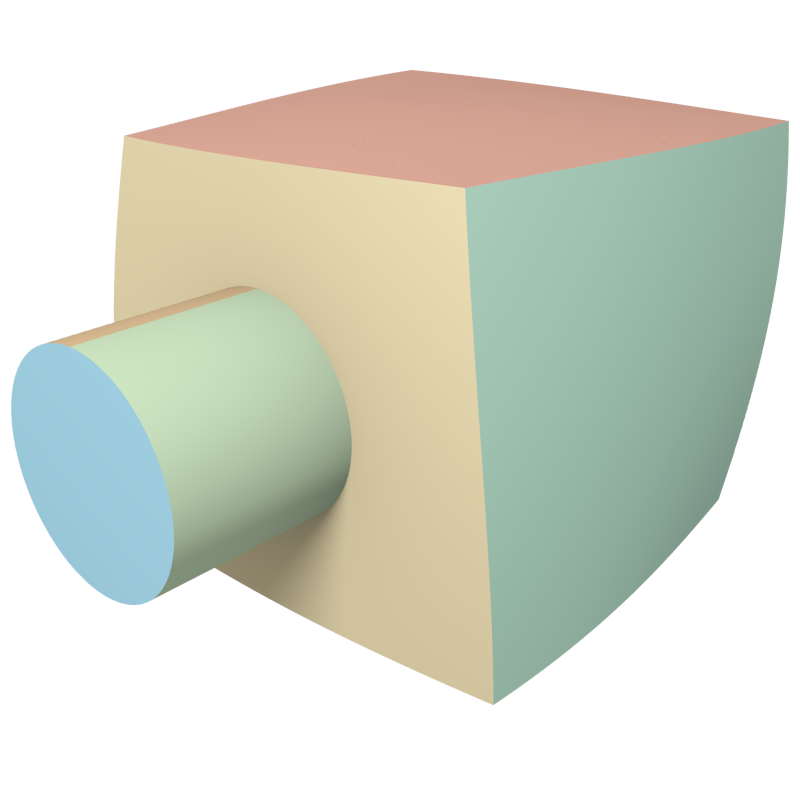
\includegraphics[width=\imagewidth]{BRep/shell}};
	%%% HIDDEN EDGES
	\node[img] at (0,0) {
\includegraphics[width=\imagewidth]{BRep/edges_hidden}};
	%%% HIDDEN VERTICES
	\DTLforeach*{dbverts}{\locx=x, \locy=y, \loca=a}{%
		\ifnum \loca = 0
			\fill[black] (\locx,\locy) circle (1.0pt);
		\fi
	}%
	%%% FACES (semi-transparent to mask hidden edges & verts)
	{\transparent{0.75}
		\node[img] at (0,0) {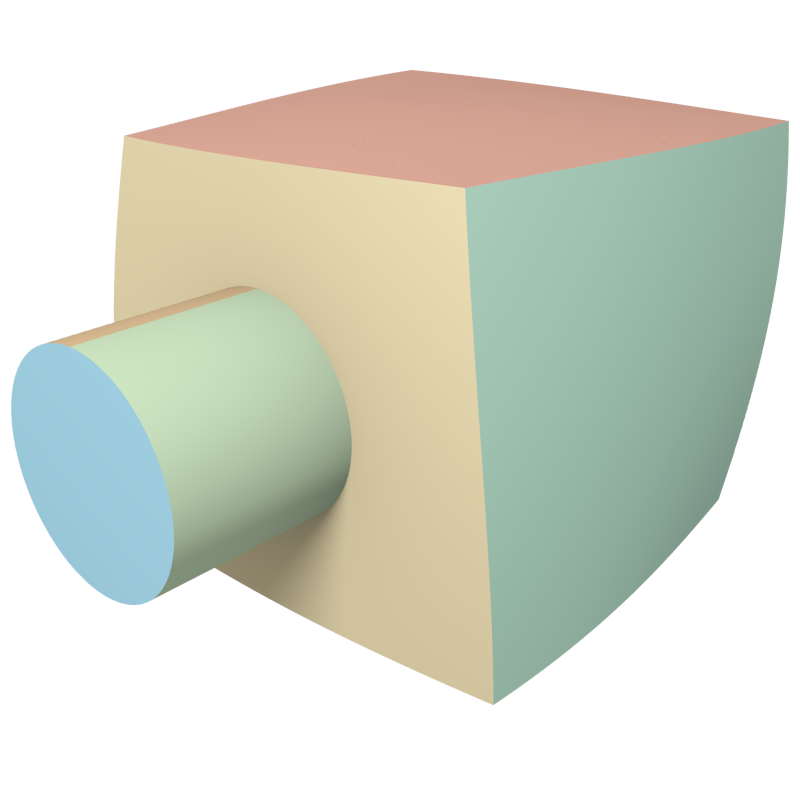
\includegraphics[width=\imagewidth]{BRep/shell}};
	}%
	%%% VISIBLE EDGES
	\node[img] at (0,0) {
\includegraphics[width=\imagewidth]{BRep/edges_visible}};
	%%% VISIBLE VERTICES
	\DTLforeach*{dbverts}{\locx=x, \locy=y, \loca=a}{%
		\ifnum \loca = 1
			\fill[black] (\locx,\locy) circle (1.0pt);
		\fi
	}%
\end{tikzpicture}
\DTLgdeletedb{dbverts}%
%%%%%%%%%%%%%%%%%%%%%%%%%%%%%%%%%%%%%%
%
%%%%%%%%%%%%%%%% FACES %%%%%%%%%%%%%%%%
\def\imfacew{44mm}
\def\ngriduv{6}
\def\vertsep{0.05}
\def\edglabsepuv{0.17}
\def\wirlabsepuv{0.18}
\def\edglabsepxyz{0.06}
\def\iniwclr{0.3}
\def\decwclr{0.3}%{0.2}
\def\uvscale{0.34}
\def\uvyshift{-0.7}
\pgfmathsetmacro\sepyshift{0.5 * (\uvyshift+\uvscale)}%
\def\surfalpha{0.04}
%
\begin{tikzpicture}[%
	x = \imfacew, y = \imfacew,
	gridtick/.style={red, fill=white, font=\tiny, inner sep=0.5pt},
	img/.style={anchor=south west, inner sep=0},
	label/.style={inner sep=1pt, font=\scriptsize},
	uvgrid/.style={black!10!white},
	curv/.style={line width=0.8pt, line cap=round},
	spacelabel/.style={anchor=north, rotate=90, inner sep=0, font=\bfseries},
	]
	\foreach \jfa/\ifa in {-1/007, 0/008, 1/002}{%
		\figbrepface{\ifa}{{1.05*\jfa - 0.5}}{{-\sepyshift}}%\hfill
	}%
	\draw[very thick, gray, dashed] 
	({-0.5*\textwidth},0) -- ++ 
	(\textwidth,0);
	\node[spacelabel] (xyzspace) at 
	({-0.5*\textwidth},{-\sepyshift+0.5}) {Espace euclidien\vphantom{Espace paramétrique}};
	\node[spacelabel] (uvspace) at 
	({-0.5*\textwidth},{\sepyshift-\uvscale}) {Espace paramétrique\vphantom{Espace euclidien}};
\end{tikzpicture}
